\section{Herangehensweise und Lösungsansatz}
\label{sec:loesungsansatz}
Um den Bildern des "images.zip"-Odners ihr Genre zuzuordnen wurde zunächst die "artists.csv"-Datei modifiziert.
Da diese die Information über die Genre eines Künstlers*in trägt ist es möglich durch sie den Bildern ihr Genre zuzuordnen.
Allerdings haben einige der Künstler*innen Bilder aus verschiedenen Genre geschaffen, weshalb in der "artists.csv"-Datei mehrere Genre unter ihrem Namen zu finden sind.
Da es alledings schwierig wäre den einzelnen Bildern der betroffenen Künstlern*innen das richtige Genre zuzuordnen, wurden jedem betroffenen Künstler*in nur ein Genre zugewiesen.
Dabei wurde das Genre welches dem Künstler*in letztendlich zugewiesen wurde zufällig aus den Genre des Künstlers*in gewählt.
Da allerdings die meisten Künstler*innen im Datensatz nur Bilder eines Genre geschaffen haben ist es nur in 12 von 50 Künstlern*innen dazu gekommen das Genre gestrichen wurden.
Die neue Datei die für jeden Künstler*in nur noch ein Genre enthält wurde "artist\_cut.csv" genannt.
Die Bilder der betroffenen Künstler*innen wurden dabei nicht verändert oder gelöscht.
\\\\
Um ein besseres Gefühl für den Datensatz zu bekommen wurde zunächst ein Jupyter Notebook \cite{Kluyver2016jupyter} erstellt in welches die "artists\_cut.csv" eingelesen wurde.
In diesem wurden nun die Anzahl der Bilder pro Genre bestimmt.
Die eingelesene Datei enthält 22 verschiedene Genre mit sehr unterschiedlicher Anzahl von Gemälden pro Genre.
Dieser Unterschied in der Anzahl von Bildern pro Genre  würde im Neuronalen Netzwerk zu einem ungleich verteilten Lernen führen.
Deshalb wurden aus dem Datensatz zunächst alle Bilder entfernt die Teil eines Genre sind welches nur 200 oder weniger Bilder beinhaltet.
Nach dem entfernen dieser Bilder bleiben noch 7343 Bilder aus 12 Genre.
\\\\
Nun wurde ein neuer Ordner erstellt in dem sich 12 weitere Ordner befinden.
Diese wurden nach den 12 Genre benannt die nach dem Aussortieren geblieben sind.
Danach wurden alle Bilder des jeweiligen Genre in den zugehörigen Ordner kopiert.
Der so erstellte Ordner "images\_genre.zip" wurde anschließend in ein neues Jupyter Notebook eingelesen.
Die Bilder wurden mit dem \textit{ImageDataGenerator} der Bibliothek \textit{Tensorflow} \cite{tensorflow2015-whitepaper} eingelesen und auf eine Größe von $100 \times 100 \times 3$ Pixeln gebracht.
Da der \textit{ImageDataGenerator} einen "Iterator" erstellt und es für uns intuitiver war mit arrays zu arbeiten haben wir darauf den Inhalt des Iterators in eine $X$ Matrix und einen $y$ Vektor überschrieben.
In der $X$ Matrix befinden sich dabei die quadratischen Bilder im RGB Format.
Der $y$ Vektor ist ein "One-Hot-Vector" auf deutsch ein "1-aus-n-Vektor".
Einige Beispiel für die verarbeiteten Bilder, die in der selben Form dem Neuronalen Netzwerk übergeben wurden, sind in Abbildung \ref{fig:beispiel_bilder} zu finden.
\begin{figure}
    \centering
    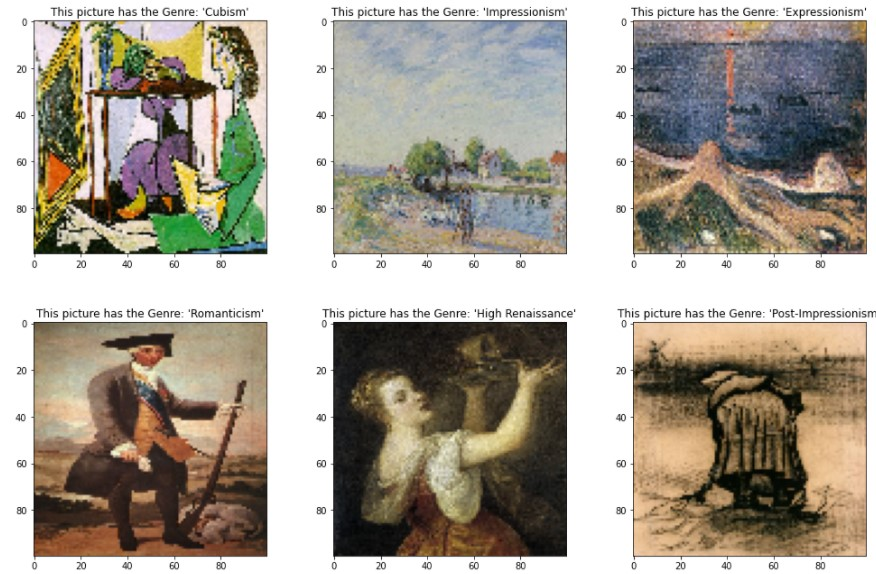
\includegraphics[width=0.7\textwidth]{content/data/beispiel.JPG}
    \caption{Einige Beispiel Bilder aus dem Testdatensatz, die in selber Form an das Netzwerk übergeben werden.}
    \label{fig:beispiel_bilder}
\end{figure}
\FloatBarrier
Da die Genre im Datensatz auf Englisch waren haben wir weiter mit den Englischen Genre Titlen gearbeitet.
Außerdem wurden, wie in dem Bild links unten in Abbildung \ref{fig:beispiel_bilder} zu sehen, manche Bilder durch das Ändern der Größe der Bilder, stark gestreckt oder gestaucht.
Zudem wird die Auflösung der Bilder durch das Ändern ihrer Größe schlechter.
Diese Limitierungen kommen durch die nur begrentzte Rechenleistung die uns zur Verfügung stand.
\subsection{Daten Aufbereitung}
Die Daten sind allerdings noch nach dem Aussortieren der Genre mit weniger als 200 Bildern sehr ungleich verteilt, wie in Abbildung \ref{fig:verteilung_daten} zu sehen ist.
So hat das Genre mit den meisten Vertretern über 1400 Bilder, wohingegen das Genre mit den wenigsten Bilder nur 260 Bilder hat.
\begin{figure}
    \centering
    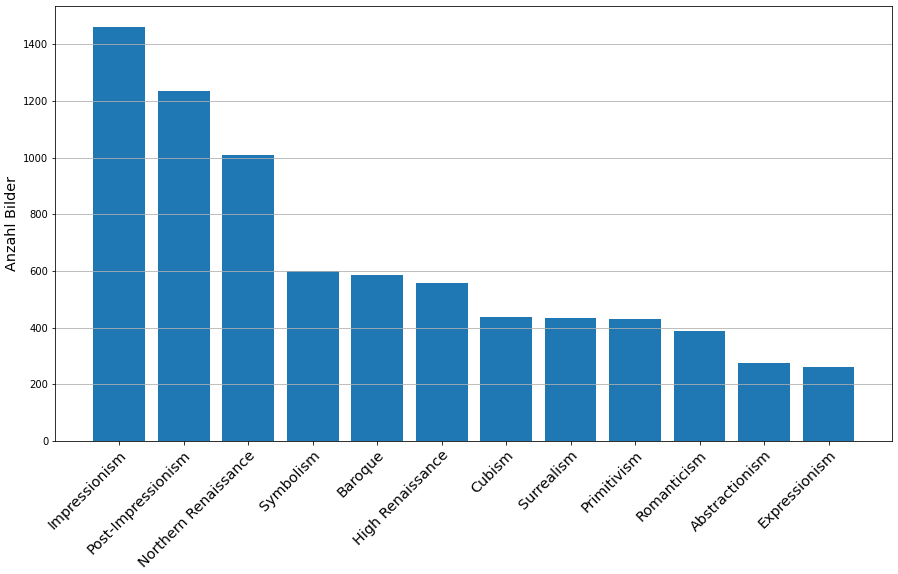
\includegraphics[width=0.55\textwidth]{content/data/Verteilung_Daten_Preprocessesing.PNG}
    \caption{Die Verteilung der Anzahl der Bilder nach Einlesen der Gerne mit mehr als 200 Bildern.}
    \label{fig:verteilung_daten}
\end{figure}
\\\\
Aus diesem Grund wurde nachdem die Daten in einen Test- und einen Trainingssatz aufgeteilt worden sind ein "Oversampling" und ein "Undersampling" durchgeführt.
Es wurden also zunächst $30\, \%$ der Bilder für den Testsatz und $70\, \%$ der Bilder für den Trainingssatz reserviert.
Es wird im späteren Verlauf weiter darauf eingegangen warum die Trennung in Test und Trainingssatz zuerst vorgenommen wurde.
\\\\
\subsubsection{Oversampling des Traingssatzes}
Wie bereits erwähnt wurde mit den Trainingssatz und dem Testsatz ein "Oversampling" und ein "Undersampling" durchgeführt.
Bei dem Oversampling wird dabei der Datensatz erweitert.
Dies wurde erreicht, indem zunächst die Anzahl von Bildern in dem Genre mit den meisten Bildern ermittelt wurde.
Im Testsatz waren dies 1023 Bilder.
Nun wurden die Bilder aus allen Genre die weniger als 1023 Bilder hatten kopiert und an das ursprüngliche Genre angehängt.
Dieser Prozess wurde für jedes unterbesetzte Genre so lange durchgeführt bis das jeweilige Genre auch 1023 Bilder hatte.
Das Ergebnis des "Oversampling" ist in Abbildung \ref{fig:oversampling} zu sehen.
Auf diese Weise tauchen in dem Datensatz, besonders in den Genre mit vorerst wenig Bildern, Bilder mehrfach auf.
Allerdings wird dadurch auch erreicht, dass die Verteilung der Anzahl der Bilder pro Genre gleich ist.
Dadurch kann das Netzwerk besser verallgemeinern.
Denn wenn der Datensatz eine ungleiche Anzahl von Bildern pro Genre haben würde, würde das Netzwerk diese Ungleichheit lernen und beim Testen zum Großteil das Genre "raten", welches im Traingssatz am häufigsten vorkam.
Dies ist natürlich unerwünscht, da das Netzwerk auf verschiedene Datensätze anwendbar seien soll, die Bilder aus den 12 gewählten Genre enthalten.
\begin{figure}
    \centering
    \caption{Ein Balkendiagramm welches die Anzahl der Bilder pro Genre zeigt. Links ist dabei der Traingssatz nach dem "Oversampling" und rechts der Traingssatz nach dem "Undersampling".}
    \begin{subfigure}{0.450\textwidth}
        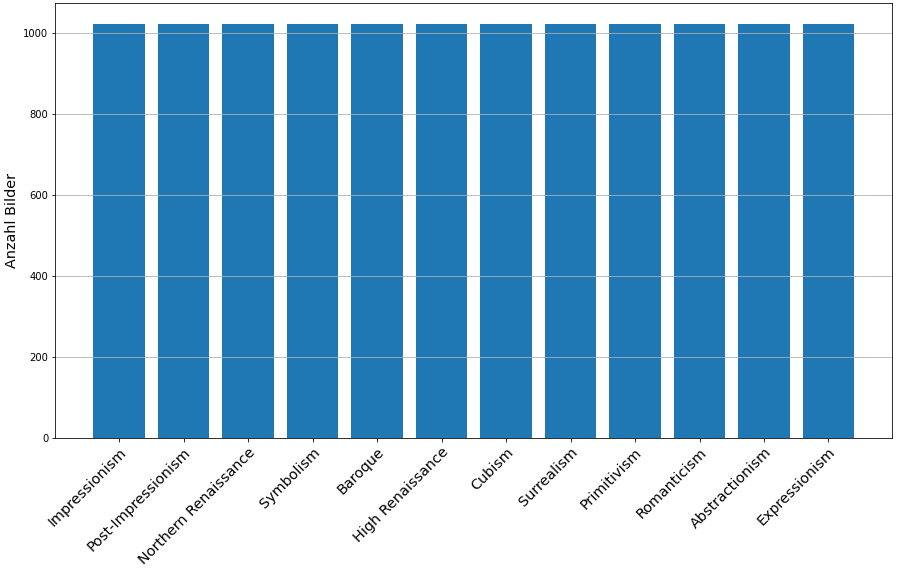
\includegraphics[width=\linewidth]{content/data/oversampling.PNG}
        \caption{Die Anzahl der Bilder nach dem "Oversampling" beträgt für jedes Genre im Traingssatz 1023.}
        \label{fig:oversampling}
    \end{subfigure}\hfil % <-- added
    \begin{subfigure}{0.450\textwidth}
        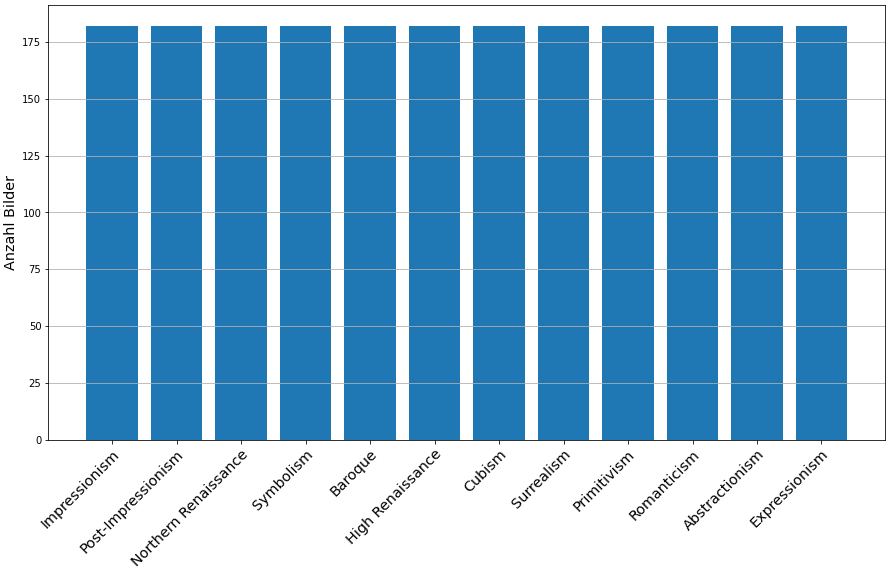
\includegraphics[width=\linewidth]{content/data/undersampling.PNG}
        \caption{Die Anzahl der Bilder nach dem "Undersampling" beträgt für jedes Genre im Traingssatz 182.}
        \label{fig:undersampling}
    \end{subfigure}\hfil % <-- added
    \label{fig:sampling}
\end{figure}
\\\\
\subsubsection{Undersampling des Traingssatzes}
Im "Undersampling" wird hingegen zum "Oversampling" der Datensatz an das Genre mit der geringsten Anzahl an Bildern angepasst.
Auf diese Anzahl wird die Anzahl der Bilder in jedem anderen Genre verringert.
Dabei werden Bilder aus dem Traingssatz gelöscht bis jedes Genre nur noch die entsprechende Anzahl an Bildern hat.
In unserem Fall hatte das Genre mit den wenisgten Bildern 182 Bilder.
Nach dem "Undersampling" hat also jedes Genre nur noch 182 Bilder.
Das Ergebnis des "Undersampling" ist in Abbildung \ref{fig:undersampling} zu sehen.
Auf diese Weise wird ebenfalls erreicht, dass die Anzahl alle Bilder in den verschiedenen Genre gleich ist.
Allerdings hat dies auch zur Folge, dass viele Bilder verloren gehen.
Da wir aber im vorhinein nicht sagen konnten welcher Traingssatz mit unserem Neuronalen Netzwerk bessere Ergebnisse liefert haben wir zunächst einen Traingssatz mit "Undersampling" und "Oversampling" erstellt.
\\\\
Sowohl der Traingssatz nach dem "Undersampling" als auch der Traingssatz nach dem "Oversampling" wurden nachdem sie erstellt wurden durchgemischt.
Dies geschieht, da sonst alle Bilder eines Genre aufeinander folgen.
Würden die Bilder also nicht gemischt werden, hätte das zur Folge, dass das Neuronale Netzwerk auch die Reihenfolge der Bilder trainiert, was zur Anwedung auf zufällige Bilder nicht erwünscht ist.

\subsubsection{Testdatensatz}
Als nächstes wurde der Testsatz bearbeitet.
Für diesen wurde nur ein "Undersampling" durchgeführt, da wir nicht wollten, dass sich in dem Testdatensatz Bilder doppelt befinden.
Nach dem "Undersampling" befanden sich im Testsatz noch 78 Bilder pro Genre.

\subsection{Das Convolutional Neural Network}
Zur Ermittlung der Genre aus den Bilddaten haben wir uns für ein "Convolutional Neural Network" (CNN) entschieden.
Der Vorteil an einem CNN ist, dass es Bildstrukturen lernt, was für unsere Problemstellung gut geeignet ist.
In Abbildung \ref{fig:model} ist der Finale Aufbau unseres Netzwerkes zu sehen.
Die Hyperparameter des Netzwerkes wurden bereits durch eine Rastersuche optimiert und sind in Abbildung \ref{fig:model_code} zu sehen.
Diese wurde für die Filter Anzahl der Convolutional Ebenen, die Größe des Kernels der Convolutional Ebenen, die Ausfallrate der Dropout Ebenen und die Anzahl der Neuronen in den dichten Ebenen und durchgeführt.
Die Ergebnisse der Rastersuche wurden anschließend in einem weiteren Jupyter Notebook abgespeichert um sie, wenn nötig, aufrufen zu können.
\\\\
Das optimierte Model aus Abbildung \ref{fig:model} besteht aus vier Convolutional Ebenen, die jeweils von einer Dropout Ebene und einer Pooling Ebene gefolgt werden.
Die Dropout Ebenen verhindern dabei die Überanpassung des Netzwerkes auf dem Traingssatz.
Auch die Pooling Ebenen verhindern die Überanpassung und ermöglicht es dem Netzwerk robuster gegen Rotationen von Bildern zu werden, was für Abstrakte Bilder vorteilhaft ist.
Außerdem reduziert es die Datenmenge was das Netzwerk schneller macht.
Nach der letzten Convolutional Ebene werden die Daten von der drei dimensionalen Matrix in eine ein dimensionalen Matrix übergeführt.
Darauf folgt eine weitere Dropout Ebene und eine dichte Ebene, die zur Reduzierung der Größe der Matrix genutzt wurde.
Abgeschlossen wird das Model durch eine dichte Ebene mit 12 Neuronen welche die Vorhersagen für die jeweiligen Bilder ausgibt.
Diese letzte dichte Ebene nuzt die \textit{softmax} Funktion als Aktivierungsfunktion, da sie einen Wertebereich zwischen 0 und 1 hat und so für die Ausgabe geeignet ist.
Die anderen Ebenen nutzen die \textit{ReLU} Funktion als Aktivierungsfunktion, aus dem Grund, dass diese keine Probleme mit schwindenen Gradtienten verursacht und sie des weiteren das Training sehr effizient macht.
Als Verlust Funktion wird die kategorische Kreuzentropie mit der Metrik Genauigkeit genutzt.
Diese ist für Mehrklassen Kategorisierungs Probleme die gängiste Verlust Funktion weswegen auch wir uns für sie entschieden haben.
Für die Metrik Genauigkeit haben wir uns entschieden, da wir möglichst viele Bilder richtig erkennen wollen ohne dabei falsche Vorhersagen zu machen.
Als "Optimizer" wurde "adam" genutzt.
\begin{figure}
    \centering
    \caption{Der Aufbau des genutzten optimierten Models. Links die Ausgabe der Funktion \textit{summary} von der Bibliothek \textit{Tensorflow} \cite{tensorflow2015-whitepaper} und rechts die Implementierung des Models als Code.}
    \begin{subfigure}{0.40\textwidth}
        \centering
        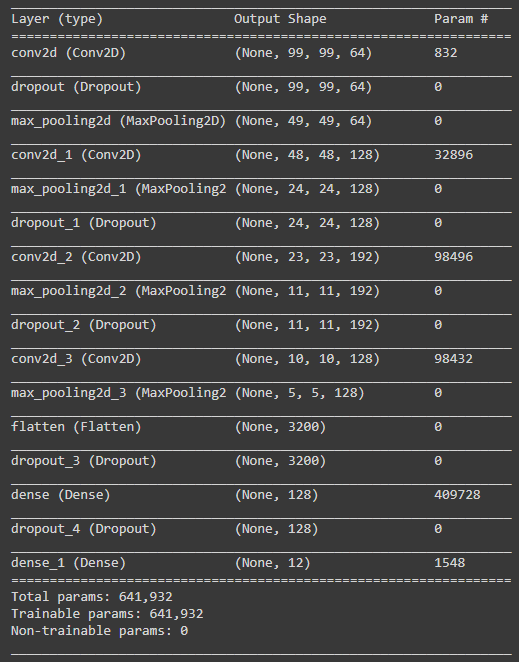
\includegraphics[width=0.6\linewidth]{content/data/model.PNG}
        \caption{Die Ausgabe der Funktion \textit{summary} auf das genutzte Model angewandt.}
        \label{fig:model_summary}
    \end{subfigure}\hfill
    \begin{subfigure}{0.40\textwidth}
        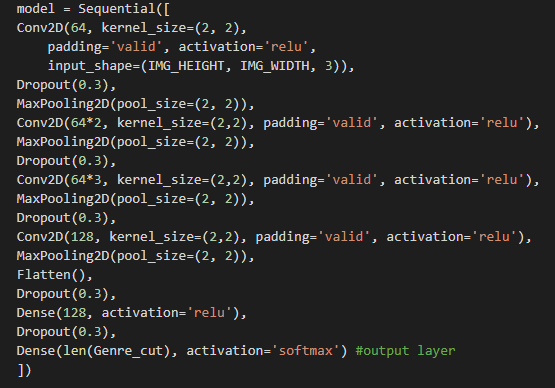
\includegraphics[width=\linewidth]{content/data/model_code.PNG}
        \caption{Die Code Implementierung des Models.}
        \label{fig:model_code}
    \end{subfigure}
    \label{fig:model}
\end{figure}
\\\\
Nachdem das Model erstellt wurde, haben wir es auf dem Trainingssatz welcher durch das "Oversampling" erweitert wurde trainiert.
Dazu haben wir einen Validierungssatz von $30\, \%$ der Trainingsdaten verwendet.
Zudem nutzen wir die Funktion \textit{EarlyStopping} aus \textit{Tensorflow} \cite{tensorflow2015-whitepaper}, um Überanpassung zu verhindern.
Wir haben mit einer maximalen Epochenzahl von 50 trainiert, \textit{EarlyStopping} hat aber nach der 35 Epoche abgebrochen.
Die Verlust Funktion des Models ist in Abbildung \ref{fig:loss} zu sehen.
Neben der Verlust Funktion ist zudem der Verlauf der Genauigkeit des Models über die 35 Epochen in Abbildung \ref{fig:accuracy} zu sehen.
Die beiden Plots wurden mit der Python Bibliothek \textit{matplotlib} \cite{matplotlib} erstellt.
Es ist zu erkennen, dass durch \textit{EarlyStopping} eine Überanpassung verhindert wurde.
Dies ist daraus zu schließen, dass sich die Funktionen auf den Validierungsdaten und auf den Trainingsdaten bei keinen der beiden Plots in Abbildung \ref{fig:training} in den letzten Epochen des Trainings weit voneinander entfernen.
\\\\
Es wurde auch ein Model auf den "Undersampling" Trainingsdaten durchgeführt.
Das so entstandene Model hat aber beim Testen wesentlich schlechter abegschnitten, weswegen im Weiteren nicht mehr weiter darauf eingegangen wird.
\begin{figure}
    \centering
    \caption{Der Verlauf der Verlust Funktion und der Genauigkeit über die 35 Trainingsepochen.}
    \begin{subfigure}{0.40\textwidth}
        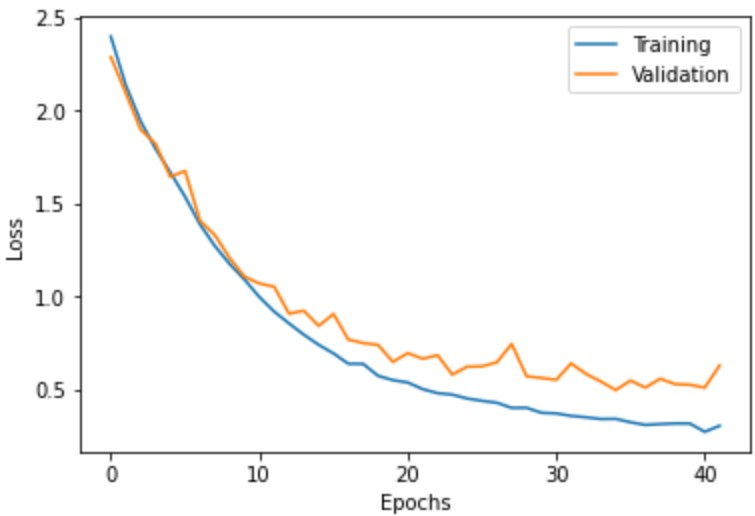
\includegraphics[width=\linewidth]{content/data/loss.JPG}
        \caption{Die Verlust Funktion des Models beim Traing über die 35 Epochen.}
        \label{fig:loss}
    \end{subfigure}\hfill
    \begin{subfigure}{0.40\textwidth}
        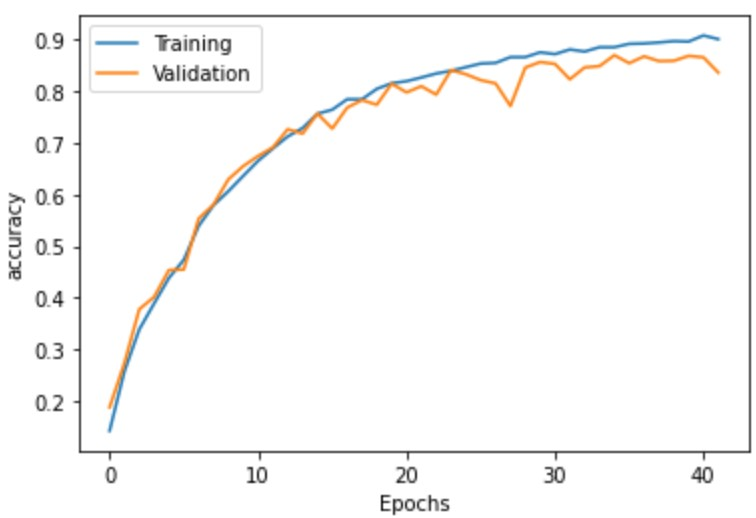
\includegraphics[width=\linewidth]{content/data/accuracy.JPG}
        \caption{Der Verlauf der Genauigkeit des Models beim Training über die 35 Epochen.}
        \label{fig:accuracy}
    \end{subfigure}
    \label{fig:training}
\end{figure}
Nach dem Trainieren sind wir direkt zum Testen übergegangen.